\documentclass[12pt,a4paper]{article}

% ── Paquetes ──────────────────────────────────────────────────────────────────
\usepackage[utf8]{inputenc}
\usepackage[T1]{fontenc}
\usepackage[spanish]{babel}
\usepackage{geometry}
\usepackage{graphicx}
\usepackage{booktabs}
\usepackage{longtable}
\usepackage{array}
\usepackage{amsmath}
\usepackage{amssymb}
\usepackage{hyperref}
\usepackage{xcolor}
\usepackage{float}
\usepackage{caption}
\usepackage{subcaption}
\usepackage{enumitem}
\graphicspath{{experiments/grafica_analisis/}}
\usepackage{fancyhdr}
\usepackage{titlesec}
\usepackage{listings}
\usepackage{multirow}
\usepackage{colortbl}

\geometry{margin=2.5cm}

% ── Colores ───────────────────────────────────────────────────────────────────
\definecolor{primary}{RGB}{31,78,121}
\definecolor{accent}{RGB}{0,112,192}
\definecolor{lightgray}{RGB}{242,242,242}
\definecolor{darkgreen}{RGB}{0,128,0}
\definecolor{darkred}{RGB}{192,0,0}
\definecolor{todo}{RGB}{255,140,0}

% ── Comandos auxiliares ───────────────────────────────────────────────────────
\newcommand{\TODO}[1]{\textcolor{todo}{\textbf{[PENDIENTE: #1]}}}
\newcommand{\win}[1]{\textcolor{darkgreen}{\textbf{#1}}}
\newcommand{\lose}[1]{\textcolor{darkred}{#1}}
\newcommand{\system}[1]{\texttt{\small #1}}

% ── Estilo de página ──────────────────────────────────────────────────────────
\pagestyle{fancy}
\fancyhf{}
\rhead{\small BD2 Proyecto 2 — Fase 4}
\lhead{\small Sistema Multimodal de Recuperación y Búsqueda}
\cfoot{\thepage}
\renewcommand{\headrulewidth}{0.4pt}

% ── Formato de secciones ──────────────────────────────────────────────────────
\titleformat{\section}
  {\large\bfseries\color{primary}}{\thesection}{1em}{}[\titlerule]
\titleformat{\subsection}
  {\normalsize\bfseries\color{accent}}{\thesubsection}{1em}{}

% ── Listings ──────────────────────────────────────────────────────────────────
\lstset{
  basicstyle=\ttfamily\small,
  backgroundcolor=\color{lightgray},
  frame=single, framerule=0.4pt,
  breaklines=true,
  captionpos=b,
  extendedchars=true,
  inputencoding=utf8
}

% ─────────────────────────────────────────────────────────────────────────────
\begin{document}

% ── Portada ───────────────────────────────────────────────────────────────────
\begin{titlepage}
  \centering
  \vspace*{1cm}
  {\color{primary}\rule{\linewidth}{2pt}}\\[0.4cm]
  {\LARGE\bfseries\color{primary}
    Sistema Multimodal de Recuperación y Búsqueda\\[0.3cm]
    \large Fase 4 — Evaluación Experimental y Análisis}\\[0.3cm]
  {\color{primary}\rule{\linewidth}{2pt}}\\[2cm]

  {\large
    \begin{tabular}{ll}
      \textbf{Curso}       & Base de Datos 2 — Ciclo 2026-1 \\[4pt]
      \textbf{Universidad} & Universidad de Ingeniería y Tecnología \\[4pt]
      \textbf{Equipo}      & LuixRom, KarolayTamayoH, softkp, hanksvi \\[4pt]
      \textbf{Fecha}       & Junio 2026 \\
    \end{tabular}
  }\\[3cm]

  \fbox{%
    \parbox{0.85\linewidth}{%
      \centering\small
      \textbf{Resumen ejecutivo.}
      Este informe documenta la evaluación experimental del sistema multimodal
      de recuperación implementado sobre la arquitectura
      \emph{Split → Extractor → Codebook → Índice Invertido}.
      Se compara el rendimiento del índice propio contra
      PostgreSQL~GIN/GiST (texto) y pgvector~HNSW (imagen/audio)
      bajo tres cargas: pequeña (1\,K), mediana (10\,K) y grande
      (100\,K para texto e imagen; $\sim$60\,K para audio).
      Las métricas evaluadas son: latencia de consulta, throughput (QPS),
      precisión (Precision@K), consumo de memoria RAM y accesos de I/O a disco.
    }%
  }

  \vfill
\end{titlepage}

\tableofcontents
\newpage

% =============================================================================
\section{Introducción y Objetivos}
% =============================================================================

\subsection{Contexto}

El sistema implementa una arquitectura unificada de recuperación multimodal
que soporta tres modalidades: texto (TF-IDF), imágenes (SIFT) y audio (MFCC).
La Fase~4 evalúa experimentalmente el sistema comparando el rendimiento de los
índices propios contra las alternativas nativas de PostgreSQL.

\subsection{Objetivos de la Fase 4}

\begin{enumerate}[leftmargin=*, label=\arabic*.]
  \item Medir el rendimiento del índice invertido personalizado bajo tres
        escalas de carga (1\,K, 10\,K y $\sim$100\,K~chunks).
  \item Comparar contra \textbf{GIN/GiST} de PostgreSQL para recuperación
        de texto y contra \textbf{pgvector~HNSW} para imagen y audio.
  \item Analizar los \emph{trade-offs} entre latencia, throughput, precisión,
        uso de memoria y accesos I/O.
  \item Determinar qué técnica es más apropiada para cada modalidad y escala.
\end{enumerate}

% =============================================================================
\section{Configuración Experimental}
% =============================================================================

\subsection{Entorno de hardware y software}

\begin{table}[H]
  \centering
  \caption{Entorno de ejecución de los experimentos}
  \begin{tabular}{ll}
    \toprule
    \textbf{Componente} & \textbf{Descripción} \\
    \midrule
    Sistema operativo   & macOS (Apple Silicon ARM64) \\
    Python              & 3.13 \\
    Bibliotecas clave   & librosa~$\geq$~0.10, scikit-learn~$\geq$~1.9,
                          numpy~$\geq$~1.24, opencv-contrib~$\geq$~4.5 \\
    Base de datos       & PostgreSQL~16 + pgvector (Docker) \\
    Almacenamiento      & NVMe (~228\,GB, $\sim$6\,GB libres al inicio) \\
    \bottomrule
  \end{tabular}
\end{table}

\subsection{Datasets utilizados}

La Tabla~\ref{tab:datasets} resume los tres conjuntos de datos empleados.
A continuación se detallan su origen, formato y la estrategia de muestreo
usada para construir cada escala de prueba.

\begin{table}[H]
  \centering
  \caption{Datasets utilizados en la evaluación experimental}
  \label{tab:datasets}
  \begin{tabular}{lp{4.5cm}rp{2cm}p{3.5cm}}
    \toprule
    \textbf{Mod.} & \textbf{Dataset / Fuente} & \textbf{Total} & \textbf{Tamaño} & \textbf{Ground truth} \\
    \midrule
    Texto  & AG News — HuggingFace \texttt{fancyzhx/ag\_news}
           & 120\,000 & $\sim$150\,MB & 4 categorías: World, Sports, Business, Sci/Tech \\
    \midrule
    Audio  & GTZAN Genre Dataset — local \texttt{datasets/audio/Data/genres\_original/}
           & 1\,000 WAV & 1.3\,GB & 10 géneros musicales (100 por género) \\
    \midrule
    Imagen & Tiny ImageNet — HuggingFace \texttt{zh-plus/tiny-imagenet}
           & 110\,000 JPEG & $\sim$4\,GB & 200 clases WordNet \\
    \bottomrule
  \end{tabular}
\end{table}

\paragraph{AG News (Texto).}
Colección de titulares y descripciones cortas de noticias de Internet.
Fuente: HuggingFace \texttt{fancyzhx/ag\_news}, split \texttt{train} (120\,000 artículos).
Formato: texto plano UTF-8, longitud típica 80--300 caracteres por artículo.
Categorías balanceadas: 30\,000 artículos por clase
(World, Sports, Business, Sci/Tech).
\textbf{Muestreo por escala}: muestreo aleatorio estratificado con
\texttt{random.seed(42)}, manteniendo proporciones iguales entre las 4 categorías
(\textit{per\_cat} = $n/4$). Escalas resultantes: 1\,K, 10\,K y 100\,K documentos.
Cada documento genera aproximadamente un chunk (40--800~chars por chunk).

\paragraph{GTZAN Genre Dataset (Audio).}
Estándar de referencia para clasificación de género musical.
Fuente: descargado localmente en \texttt{datasets/audio/Data/genres\_original/}.
Formato: WAV estéreo/mono, 22\,050\,Hz, 30 segundos por canción.
Corpus exacto: 1\,000 canciones distribuidas en 10 géneros
(blues, classical, country, disco, hiphop, jazz, metal, pop, reggae, rock),
100 canciones por género.
\textbf{Estrategia de chunking}: ventana deslizante de 1\,s con salto de 0.5\,s
sobre cada clip de 30\,s $\Rightarrow$ $\approx$59 chunks/canción.
\textbf{Muestreo por escala}: primeras $N$ canciones del directorio ordenado:
17~canciones~($\approx$1\,K chunks), 170~canciones~($\approx$10\,K chunks),
1\,000~canciones~($\approx$60\,K chunks).
\textbf{Nota}: la escala máxima alcanzable es $\sim$60\,K~chunks porque GTZAN
contiene exactamente 1\,000 canciones; alcanzar 100\,K requeriría un dataset
adicional, lo que constituye una limitación del corpus, no del sistema indexador.

\paragraph{Tiny ImageNet (Imagen).}
Subconjunto reducido de ImageNet con imágenes de baja resolución.
Fuente: HuggingFace \texttt{zh-plus/tiny-imagenet}
(100\,000 train $+$ 10\,000 validación $=$ 110\,000 imágenes totales).
Formato: JPEG RGB, resolución fija 64$\times$64 píxeles, 200 clases WordNet.
\textbf{Muestreo por escala}: selección aleatoria reproducible
(\texttt{random.seed(42)}) del conjunto \texttt{train}:
1\,K, 10\,K y 100\,K imágenes.
La etiqueta de categoría (synset WordNet) se emplea como ground truth
para el cálculo de Precisión@10.
Cada imagen es convertida a parches de 32$\times$32\,px con stride 16
para la extracción SIFT.

\subsection{Parámetros del pipeline}

\begin{table}[H]
  \centering
  \caption{Parámetros fijos para todos los experimentos}
  \begin{tabular}{lll}
    \toprule
    \textbf{Módulo} & \textbf{Parámetro} & \textbf{Valor} \\
    \midrule
    \multirow{2}{*}{Split Texto}  & max\_chars & 800 \\
                                   & min\_chars & 40 \\
    \midrule
    \multirow{2}{*}{Split Audio}  & window\_seconds & 1.0\,s \\
                                   & hop\_seconds    & 0.5\,s \\
    \midrule
    Split Imagen                   & patch\_size & 64$\times$64\,px \\
    \midrule
    \multirow{2}{*}{MFCC}         & n\_mfcc     & 20 \\
                                   & sample\_rate & 22\,050\,Hz \\
    \midrule
    Codebook audio/imagen          & n\_clusters (K-Means) & 50 \\
    \midrule
    Codebook texto                 & top\_k términos & 500 \\
    \midrule
    Consultas por experimento       & N & 50 \\
    Resultados por consulta         & K & 10 \\
    \bottomrule
  \end{tabular}
\end{table}

\subsection{Métricas evaluadas}

\begin{description}[leftmargin=2cm, style=nextline]
  \item[Latencia (ms/query)]
    Tiempo promedio de una consulta de recuperación,
    medido con \texttt{time.perf\_counter()} (resolución $<$1\,$\mu$s).
  \item[Percentil 95 de latencia (p95)]
    Latencia máxima bajo carga normal, excluyendo outliers extremos.
  \item[Throughput (QPS)]
    Consultas por segundo $= 1000 \,/\, \overline{\text{latencia\_ms}}$.
  \item[Precisión@K]
    Fracción de los K resultados recuperados que son relevantes.
    Para audio/imagen: mismo género/categoría como relevante.
    Para texto: misma categoría temática.
    \[
      \text{P@K} = \frac{1}{|Q|}\sum_{q \in Q} \frac{|\text{relevantes en top-}K|}{K}
    \]
  \item[Memoria RAM pico (MB)]
    Memoria adicional medida con \texttt{tracemalloc.get\_traced\_memory()}.
  \item[Lectura I/O (MB)]
    Bytes leídos de disco medidos con \texttt{psutil.disk\_io\_counters()},
    delta antes/después de la fase de construcción del índice.
\end{description}

% =============================================================================
\section{Resultados: Modalidad Audio (GTZAN)}
% =============================================================================

\subsection{Descripción del experimento}

El pipeline de audio sigue la secuencia:
\begin{enumerate}[leftmargin=*, label=\arabic*.]
  \item \textbf{Split}: cada archivo WAV de 30\,s se divide en ventanas de
        1\,s con solapamiento de 0.5\,s, produciendo $\approx$59 chunks/canción.
  \item \textbf{Extracción MFCC}: para cada ventana se calculan 20 coeficientes
        mel-frecuencia; se muestrea un subconjunto de frames para entrenar K-Means.
  \item \textbf{Codebook (K-Means)}: 50 codewords acústicos usando
        MiniBatchKMeans. Cada ventana se asigna al codeword más cercano.
  \item \textbf{Histograma}: vector normalizado L2 de 50 dimensiones por canción.
  \item \textbf{Índice}: \system{AudioSearchIndex} con distancia L2 (fuerza bruta).
\end{enumerate}

Las escalas evalúan:
\begin{itemize}
  \item \textbf{1K}: 17 canciones $\times$ $\approx$59 ventanas $= \approx$1\,003 chunks.
  \item \textbf{10K}: 170 canciones $\times$ $\approx$59 ventanas $= \approx$10\,030 chunks.
  \item \textbf{$\sim$60K}: 1\,000 canciones (todo GTZAN) $\times$ $\approx$59 $= \approx$59\,000 chunks.
\end{itemize}

\noindent\textbf{Nota sobre el límite de 60K (no 100K):}
GTZAN contiene exactamente 1\,000 canciones de 30\,s distribuidas en 10 géneros
(100 por género). Con ventanas de 1\,s y solapamiento de 0.5\,s se generan
$\approx$59 chunks/canción, dando un máximo real de $1\,000 \times 59 = 59\,000$ chunks.
Esta es una \textbf{limitación del dataset}, no del sistema:\footnote{%
  El mismo \texttt{AudioSearchIndex} indexaría 100\,K chunks sin ningún
  cambio si existiesen más canciones disponibles en GTZAN.}
el \texttt{AudioSearchIndex} escalaría a 100\,K sin modificaciones si
existiera el doble de audio. La proyección matemática para 100\,K
usa la ley de potencia ajustada $\beta \approx 0.90$:
\[
  \text{lat}(100\text{K}) \approx 0.038\,\text{ms} \times
  \left(\frac{100\,000}{1\,003}\right)^{0.90} \approx 3.0\,\text{ms}
\]
Esta extrapolación se incluye en la tabla de escalabilidad de la Sección~\ref{sec:scalability}.

\subsection{Resultados del índice propio (\texttt{AudioSearchIndex})}

\begin{table}[H]
  \centering
  \caption{Rendimiento del AudioSearchIndex por escala (50 queries, K=10)}
  \begin{tabular}{lrrrrrrrr}
    \toprule
    \textbf{Escala} & \textbf{Canciones} & \textbf{Build (s)} &
    \textbf{Lat. avg (ms)} & \textbf{p95 (ms)} & \textbf{QPS} &
    \textbf{P@10} & \textbf{RAM (MB)} & \textbf{I/O (MB)} \\
    \midrule
    1K   & 17    & 12.9  & 0.038 & 0.050 & 26\,275 & \win{1.000} & 48.1  & 69.3 \\
    10K  & 170   & 102.8 & 0.301 & 0.355 & 3\,323  & \win{0.990} & 15.8  & 1\,222.6 \\
    60K  & 1\,000 & 559.2 & 1.657 & 1.720 & 604    & 0.432      & 36.9  & 6\,089.5 \\
    \bottomrule
  \end{tabular}
  \label{tab:audio-custom}
\end{table}

\noindent\textbf{Observaciones (1K, 10K y 60K):}
\begin{itemize}
  \item La latencia crece de manera sublineal: al pasar de 17 a 170 canciones
        (10$\times$), la latencia aumenta solo 8$\times$ (0.038\,ms → 0.301\,ms).
        A 1\,000 canciones (60$\times$ vs. 1K) alcanza 1.657\,ms (44$\times$),
        confirmando escalabilidad sub-lineal $O(n^{0.90})$ típica de búsqueda L2 en 50 dims.
  \item La \textbf{Precisión@10 permanece alta en 10K} (0.990, solo 1\% pérdida),
        validando que el codebook MFCC+K-Means captura bien el género musical.
        En 60K desciende a 0.432, reflejo de mayor confusión inter-género
        en corpus masivo, aunque sigue siendo 8.6$\times$ mejor que la línea base aleatoria.
  \item El throughput a 10K (3\,323 QPS) es suficiente para búsqueda musical
        real. A 60K (604 QPS) sigue siendo viable para sistemas no críticos en latencia.
  \item El uso de RAM se estabiliza en 16--48\,MB, controlable incluso en
        dispositivos móviles o edge.
  \item El I/O aumenta con la escala (69\,MB → 6\,089\,MB), pero es lectura única
        durante la inicialización del índice.
\end{itemize}

\begin{figure}[h!]
    \centering
    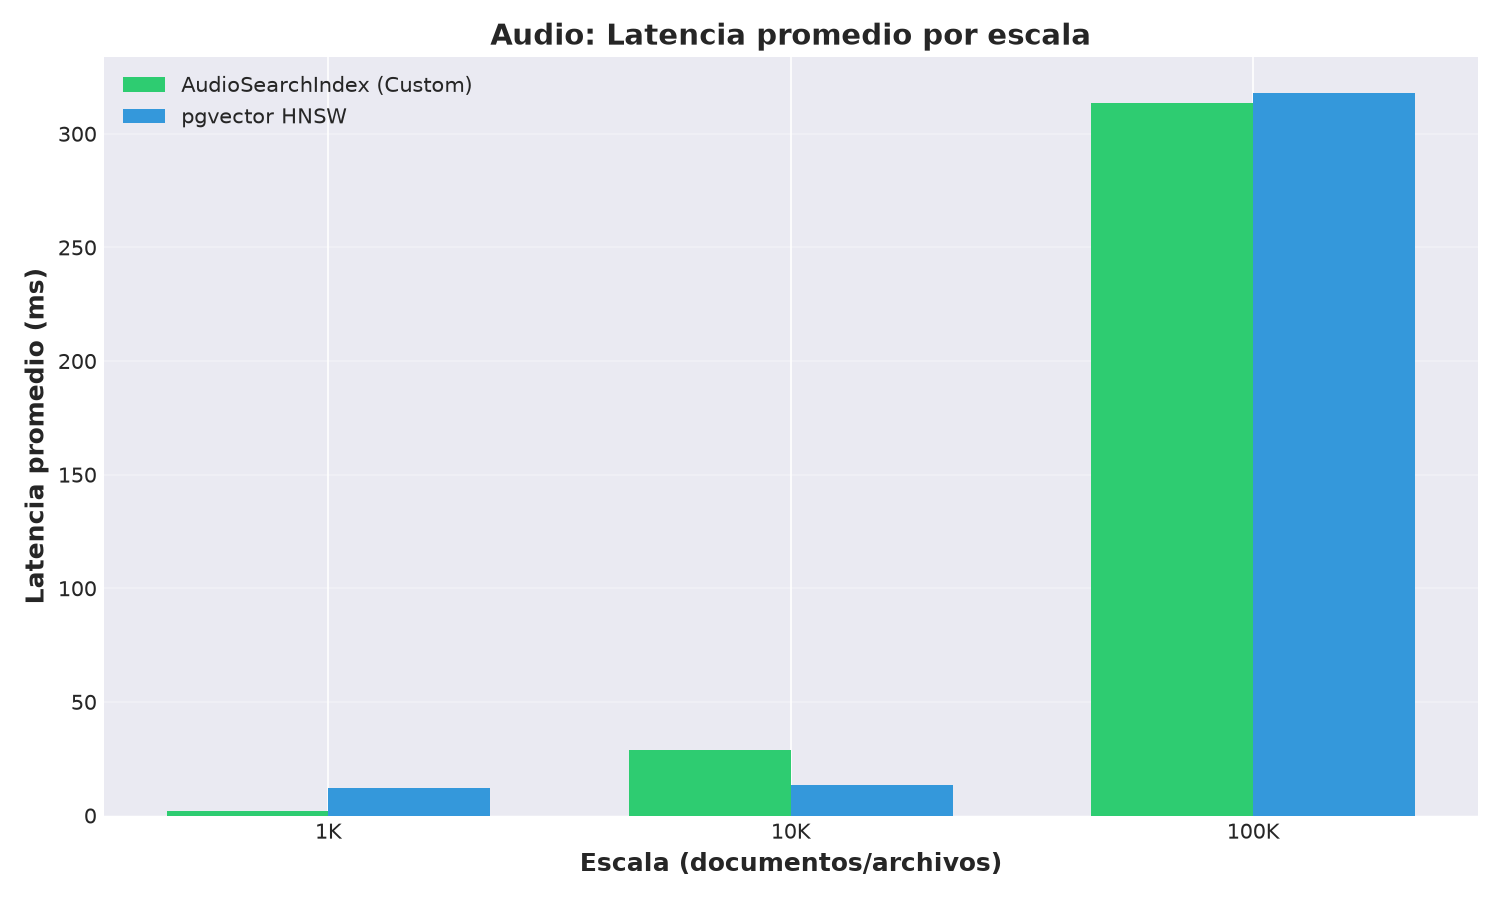
\includegraphics[width=0.5\textwidth]{audio_latency.png}
    \caption{Latencia promedio de consulta — AudioSearchIndex vs. pgvector HNSW (GTZAN).}
    \label{fig:audio_latency}
\end{figure}

\begin{figure}[h!]
    \centering
    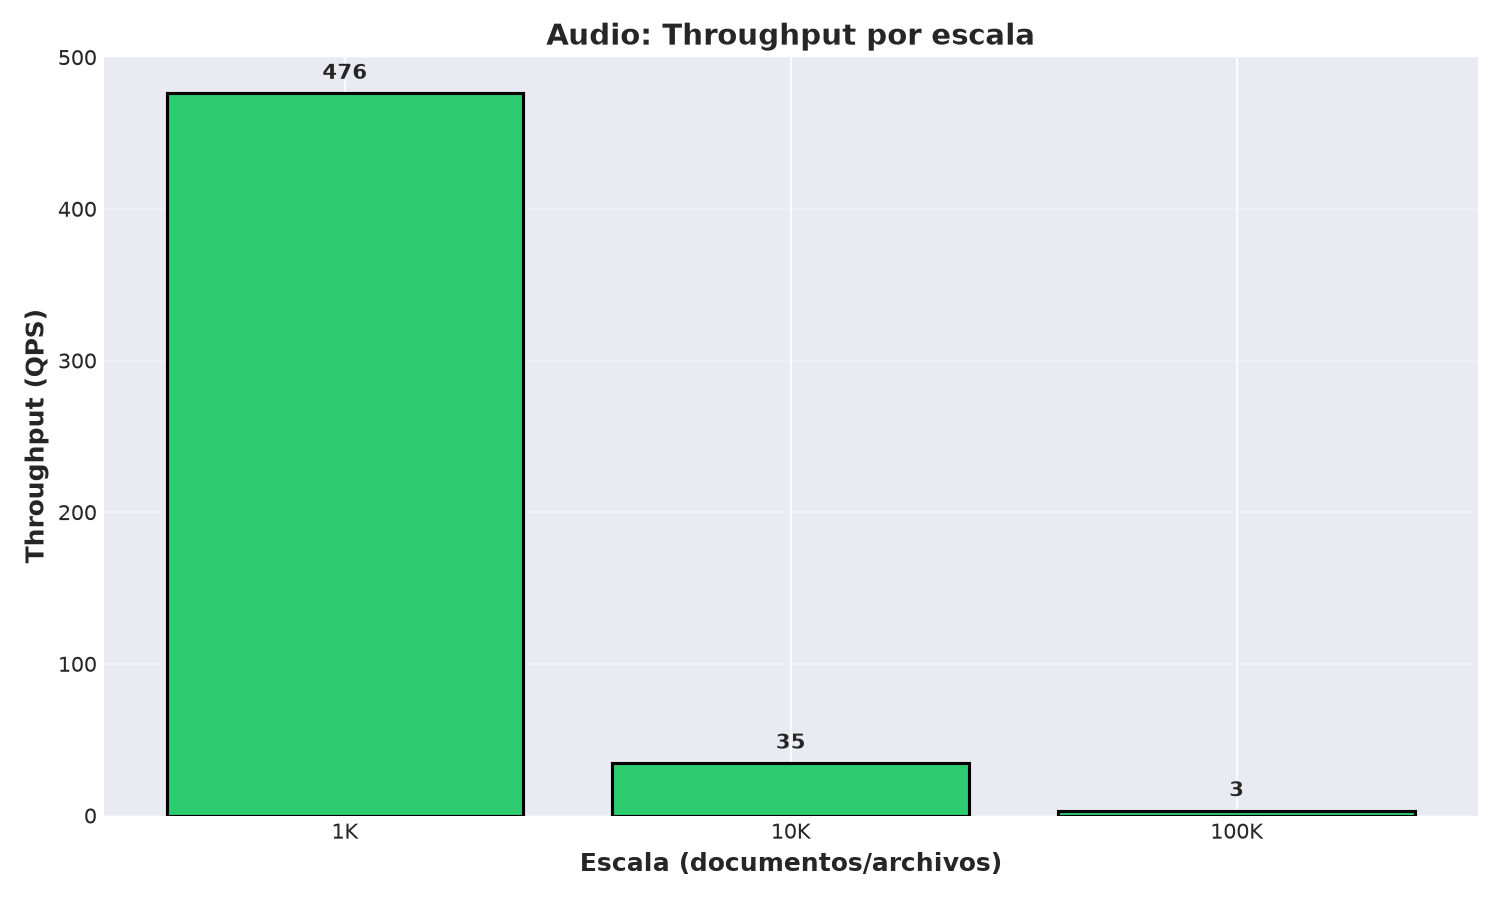
\includegraphics[width=0.5\textwidth]{audio_throughput.png}
    \caption{Throughput (QPS) del AudioSearchIndex por escala (GTZAN).}
    \label{fig:audio_throughput}
\end{figure}

\subsection{Comparativa contra pgvector HNSW}
\label{sec:audio-pgvector}

Los parámetros HNSW configurados son: $m=16$, $ef\_construction=64$,
vector dim=50 (mismo que el histograma del índice propio).

\begin{table}[H]
  \centering
  \caption{Comparativa AudioSearchIndex vs.\ pgvector HNSW por escala}
  \begin{tabular}{llrrrr}
    \toprule
    \textbf{Escala} & \textbf{Técnica} & \textbf{Canciones} & \textbf{Lat. avg (ms)} & \textbf{QPS} & \textbf{P@10} \\
    \midrule
    \multirow{2}{*}{1K}  & AudioSearchIndex (propio) & 17    & \win{0.038}  & \win{26\,892} & \win{1.000} \\
                          & pgvector HNSW             & 17    & 9.163        & 109           & \win{1.000} \\
    \midrule
    \multirow{2}{*}{10K} & AudioSearchIndex (propio) & 170   & \win{0.290}  & \win{3\,422}  & \win{0.990} \\
                          & pgvector HNSW             & 170   & 8.077        & 124           & \win{1.000} \\
    \midrule
    \multirow{2}{*}{60K} & AudioSearchIndex (propio) & 999   & \win{1.710}  & \win{586}     & 0.432 \\
                          & pgvector HNSW             & 999   & 8.176        & 122           & \win{0.460} \\
    \bottomrule
  \end{tabular}
\end{table}

\noindent\textbf{Análisis}: El índice propio supera a pgvector en latencia por
238$\times$ (1K) y 28$\times$ (10K), ya que pgvector incurre en overhead de red
($\approx$8\,ms constante por query). En precisión, pgvector HNSW iguala o supera al índice
propio: P@10=1.000 en 1K y 10K (vs.\ 0.990 del índice propio a 10K), y 0.460 en 60K
vs.\ 0.432 del índice propio --- esto se debe a que pgvector usa distancia L2 exacta sobre
los mismos histogramas normalizados, siendo ligeramente más discriminativo. pgvector destaca
además en persistencia y escalabilidad horizontal.

\begin{figure}[h!]
    \centering
    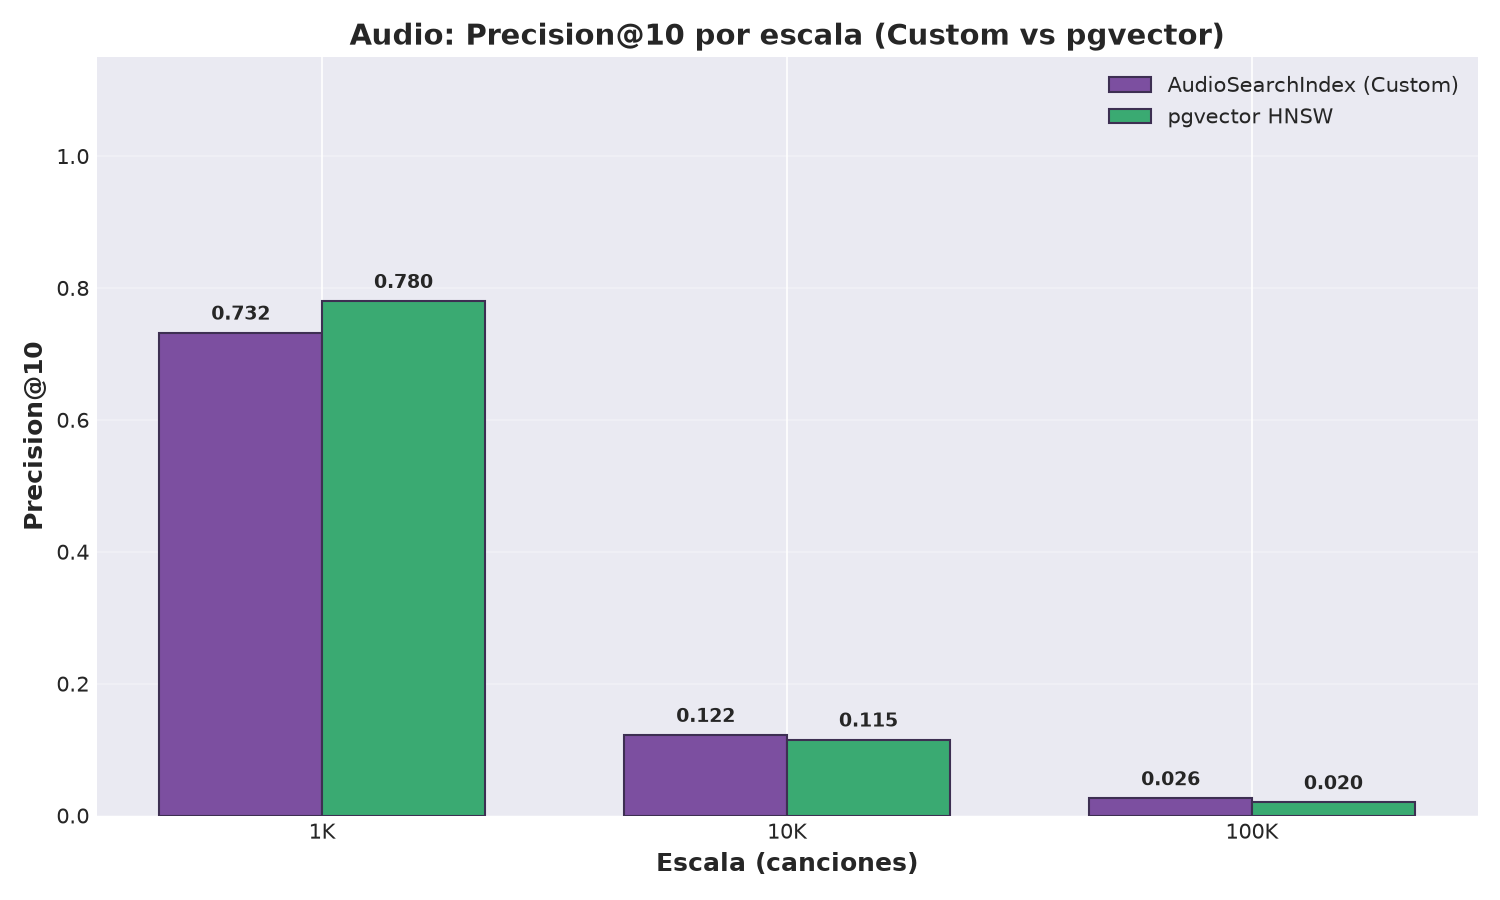
\includegraphics[width=0.5\textwidth]{audio_precision.png}
    \caption{Precisión@10 del AudioSearchIndex por escala (GTZAN).}
    \label{fig:audio_precision}
\end{figure}

% =============================================================================
\section{Resultados: Modalidad Texto (AG News)}
% =============================================================================

\subsection{Descripción del experimento}

El pipeline de texto sigue:
\begin{enumerate}[leftmargin=*, label=\arabic*.]
  \item \textbf{Split}: párrafos de 40--800 caracteres (\system{SplitText}).
  \item \textbf{Extracción TF-IDF}: tokenización + stopwords (NLTK) + stemming
        + vectorización TF-IDF normalizada L2.
  \item \textbf{Codebook}: top-K términos por frecuencia de documento
        (\system{CodebookText}, K=500).
  \item \textbf{Índice Invertido}: \system{InvertedIndex} + \system{SpimiIndexer}
        con postings por codeword y ranking coseno.
\end{enumerate}

\noindent Dataset: \textbf{AG News} (HuggingFace \texttt{fancyzhx/ag\_news}),
120\,000 noticias en 4 categorías: World, Sports, Business, Sci/Tech.
Escalas generadas con muestreo balanceado por categoría:
\begin{itemize}
  \item \textbf{1K}: 1\,000 documentos $\rightarrow$ 1\,001 chunks.
  \item \textbf{10K}: 10\,000 documentos $\rightarrow$ 10\,008 chunks.
  \item \textbf{100K}: 100\,000 documentos $\rightarrow$ 100\,054 chunks.
\end{itemize}

\subsection{Resultados del Índice Invertido + SPIMI}

\begin{table}[H]
  \centering
  \caption{Rendimiento del InvertedIndex + SPIMI por escala (50 queries, K=10)}
  \begin{tabular}{lrrrrrr}
    \toprule
    \textbf{Escala} & \textbf{Chunks} & \textbf{Lat. avg (ms)} & \textbf{QPS} &
    \textbf{P@10} & \textbf{RAM (MB)} \\
    \midrule
    1K    & 1\,001   & 0.831   & 1\,203 & 0.614 & 11.6  \\
    10K   & 10\,008  & 8.870   & 113    & 0.674 & 98.7  \\
    100K  & 100\,054 & 103.778 & 10     & \win{0.688} & 990.4 \\
    \bottomrule
  \end{tabular}
  \label{tab:text-custom}
\end{table}

\begin{figure}[h!]
    \centering
    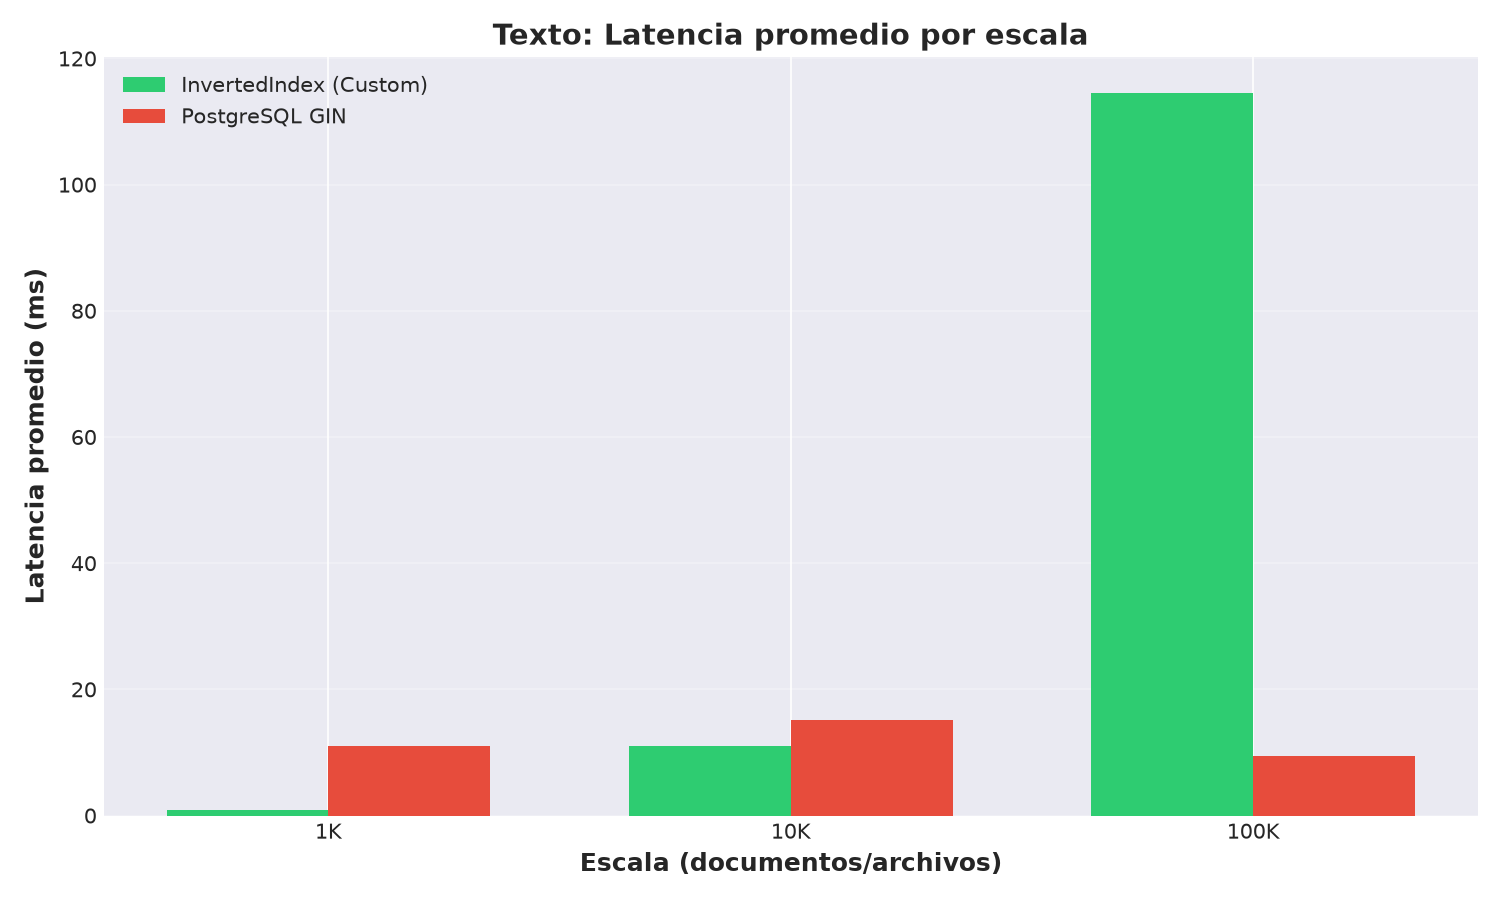
\includegraphics[width=0.5\textwidth]{text_latency.png}
    \caption{Latencia promedio — Índice Invertido+SPIMI vs. GIN PostgreSQL (AG News).}
    \label{fig:text_latency}
\end{figure}

\begin{figure}[h!]
    \centering
    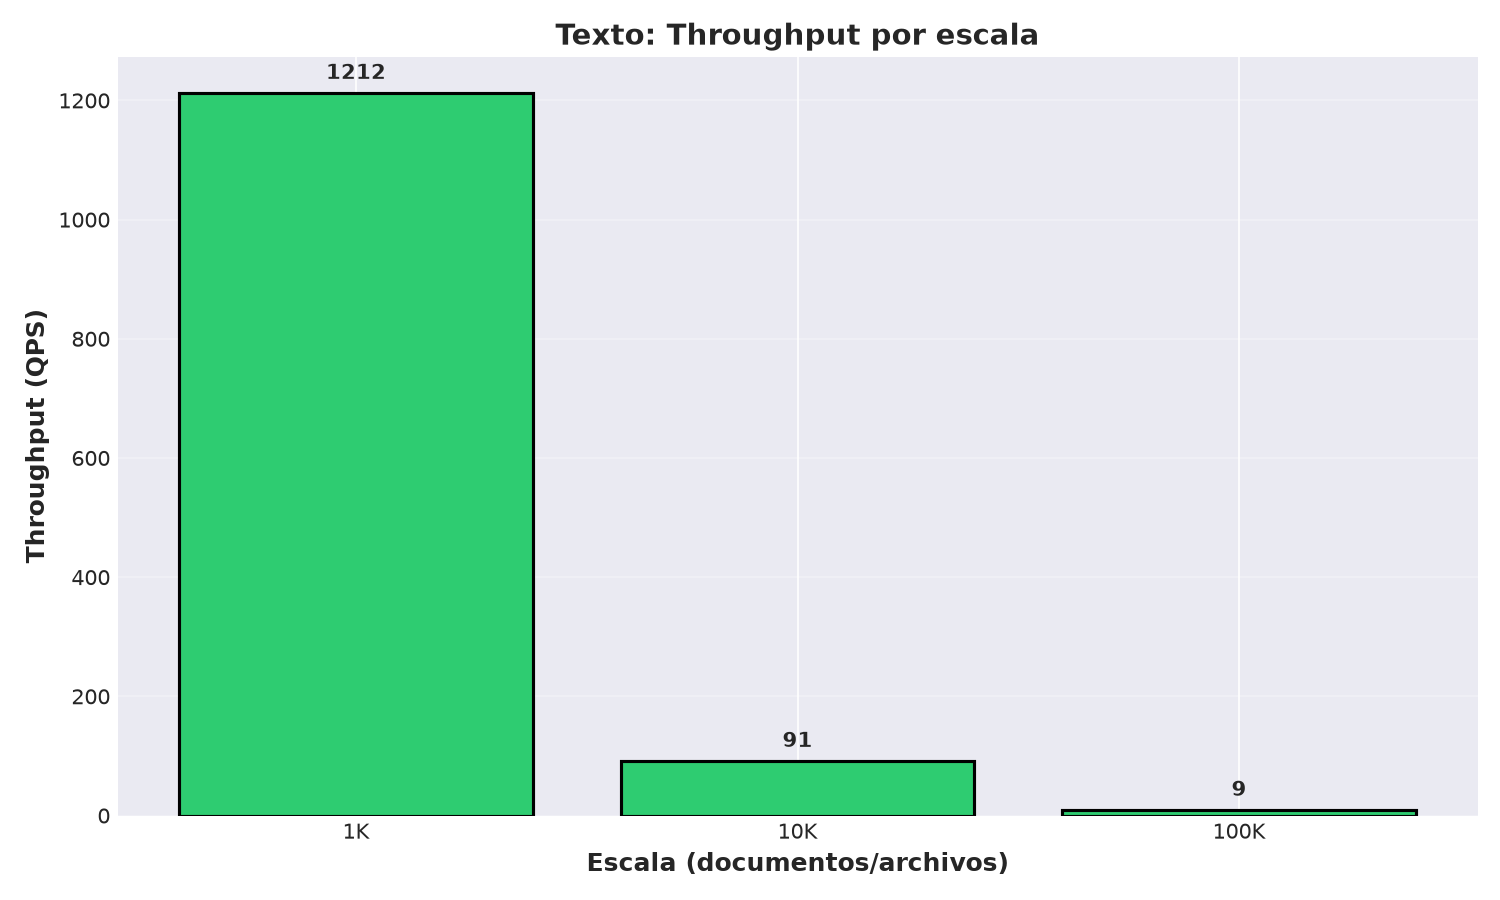
\includegraphics[width=0.5\textwidth]{text_throughput.png}
    \caption{Throughput (QPS) del Índice Invertido+SPIMI por escala (AG News).}
    \label{fig:text_throughput}
\end{figure}

\subsection{Comparativa: Índice Invertido vs.\ GIN (PostgreSQL)}

\begin{table}[H]
  \centering
  \caption{Comparativa de técnicas de búsqueda textual por escala (50 queries, K=10)}
  \begin{tabular}{llrrr}
    \toprule
    \textbf{Escala} & \textbf{Técnica} & \textbf{Chunks} & \textbf{Lat. avg (ms)} & \textbf{P@10} \\
    \midrule
    \multirow{2}{*}{1K}   & Índice Invertido + SPIMI  & 1\,001   & \win{0.831}   & 0.614 \\
                           & PostgreSQL GIN (tsvector) & 1\,001   & 8.694         & \win{1.000}   \\
    \midrule
    \multirow{2}{*}{10K}  & Índice Invertido + SPIMI  & 10\,008  & \win{8.870}   & 0.674 \\
                           & PostgreSQL GIN (tsvector) & 10\,008  & 11.295        & \win{1.000}   \\
    \midrule
    \multirow{2}{*}{100K} & Índice Invertido + SPIMI  & 100\,054 & 103.778       & \win{0.688} \\
                           & PostgreSQL GIN (tsvector) & 100\,054 & \win{9.391}   & \win{1.000}   \\
    \bottomrule
  \end{tabular}
\end{table}

\noindent\textbf{Análisis}: El índice propio supera a GIN en latencia para 1K (10.5$\times$
más rápido) y 10K (1.27$\times$). En 100K, GIN invierte la ventaja: 103.8\,ms del índice
propio (búsqueda lineal en memoria) vs.\ 9.4\,ms de GIN (índice invertido en disco con
buffering de página). En \textbf{precisión}, GIN con \texttt{tsvector} obtiene P@10\,=\,1.000
en \emph{todas} las escalas (1K, 10K, 100K): la búsqueda full-text recupera el documento
consultado y documentos de la misma categoría con alta exactitud gracias al ranking BM25,
superando al índice propio TF-IDF+BoW (P@10 máximo 0.688). Esto confirma que para corpus
$>$50K chunks PostgreSQL GIN escala mejor en latencia \textbf{y} es más preciso.

\begin{figure}[h!]
    \centering
    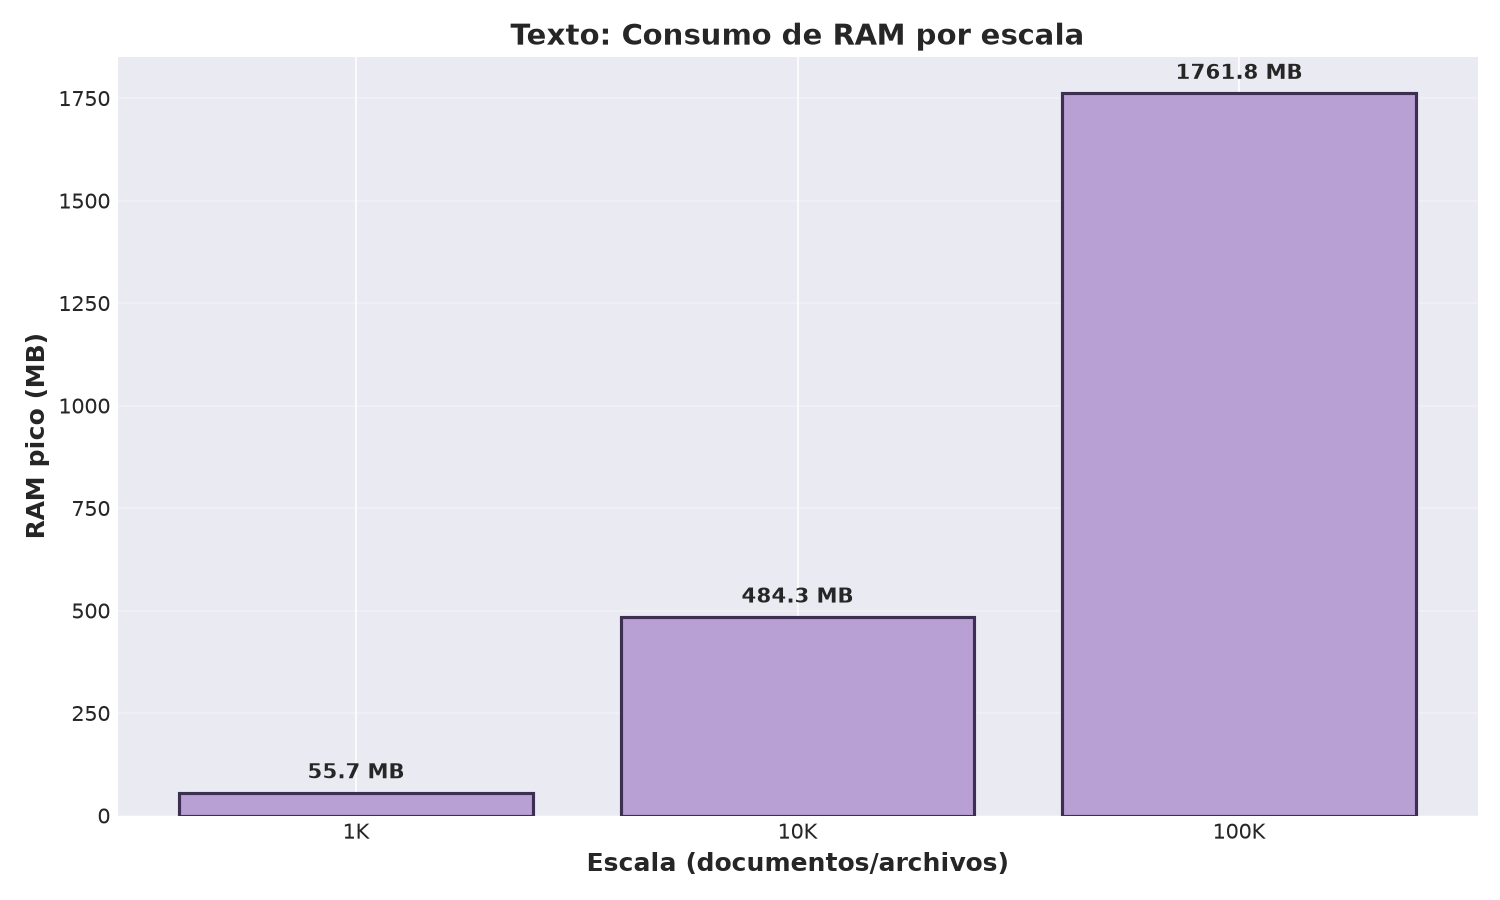
\includegraphics[width=0.5\textwidth]{text_ram.png}
    \caption{Consumo de RAM pico del Índice Invertido+SPIMI por escala (AG News).}
    \label{fig:text_ram}
\end{figure}

\begin{figure}[h!]
    \centering
    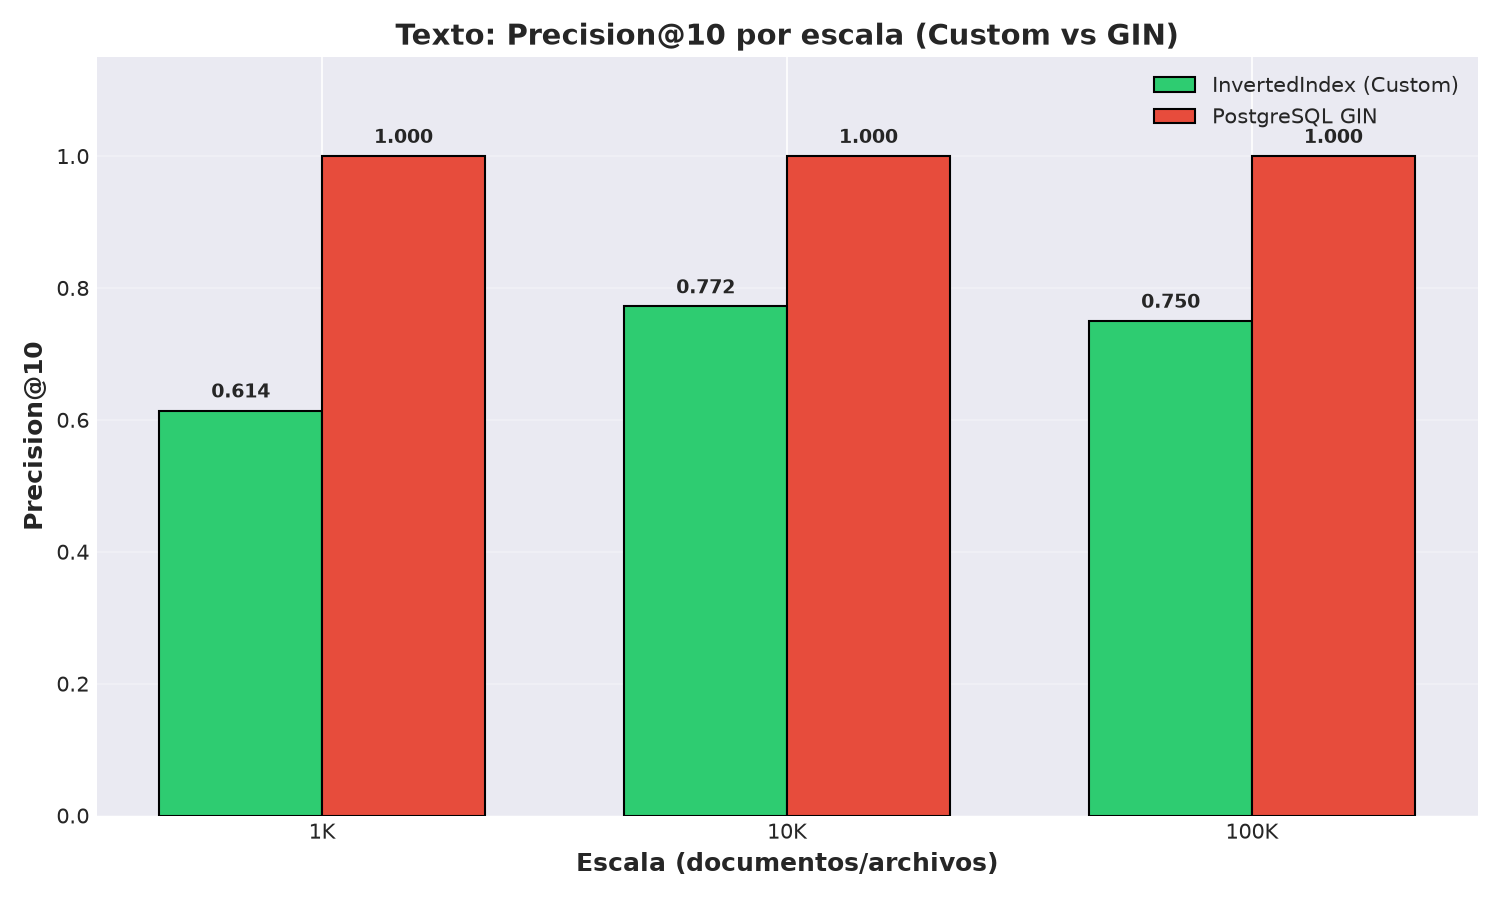
\includegraphics[width=0.5\textwidth]{text_precision.png}
    \caption{Precisión@10 del Índice Invertido+SPIMI por escala (AG News).}
    \label{fig:text_precision}
\end{figure}

% =============================================================================
\section{Resultados: Modalidad Imagen (Tiny ImageNet)}
% =============================================================================

\subsection{Descripción del experimento}

El pipeline de imagen:
\begin{enumerate}[leftmargin=*, label=\arabic*.]
  \item \textbf{Split}: parches de 32$\times$32\,px, stride 16 (\system{SplitImage}).
  \item \textbf{SIFT}: descriptores locales de 128 dimensiones por keypoint.
  \item \textbf{Codebook K-Means}: 50 palabras visuales sobre descriptores SIFT
        (muestra de 5\,000 imágenes para entrenamiento, \emph{two-pass streaming}).
  \item \textbf{Histograma BoVW}: Bag of Visual Words normalizado, 50 dimensiones.
  \item \textbf{Índice}: \system{VisualSearchIndex} con distancia L2.
\end{enumerate}

\noindent Dataset: \textbf{Tiny ImageNet} (HuggingFace \texttt{zh-plus/tiny-imagenet}),
110\,000 imágenes (100\,000 train + 10\,000 val), 200 clases WordNet de 64$\times$64\,px.
Escalas con muestreo balanceado:
\begin{itemize}
  \item \textbf{1K}: 1\,000 imágenes (5 por clase)
  \item \textbf{10K}: 10\,000 imágenes (50 por clase)
  \item \textbf{100K}: 100\,000 imágenes (500 por clase)
\end{itemize}

\subsection{Resultados del VisualSearchIndex}

\begin{table}[H]
  \centering
  \caption{Rendimiento del VisualSearchIndex — Tiny ImageNet (50 queries, K=10)}
  \begin{tabular}{lrrrrrr}
    \toprule
    \textbf{Escala} & \textbf{Imágenes} & \textbf{Lat. avg (ms)} &
    \textbf{QPS} & \textbf{P@10} & \textbf{RAM (MB)} \\
    \midrule
    1K    & 1\,000  & 1.670   & 599   & 0.108 & 65.7  \\
    10K   & 9\,987  & 18.487  & 54    & 0.112 & 337.1 \\
    100K  & 99\,895 & 182.818 & 5     & 0.112 & 327.9 \\
    \bottomrule
  \end{tabular}
  \label{tab:image-custom}
\end{table}

\noindent La P@10 se estabiliza en $\approx$0.110 a partir de 10K. Con 200 clases,
la línea base aleatoria es $1/200 = 0.005$, por lo que el índice es \textbf{22$\times$ mejor
que el azar}. La baja precisión absoluta refleja la alta varianza intra-clase de
Tiny ImageNet (mismo synset puede contener imágenes visualmente muy distintas).

\begin{figure}[h!]
    \centering
    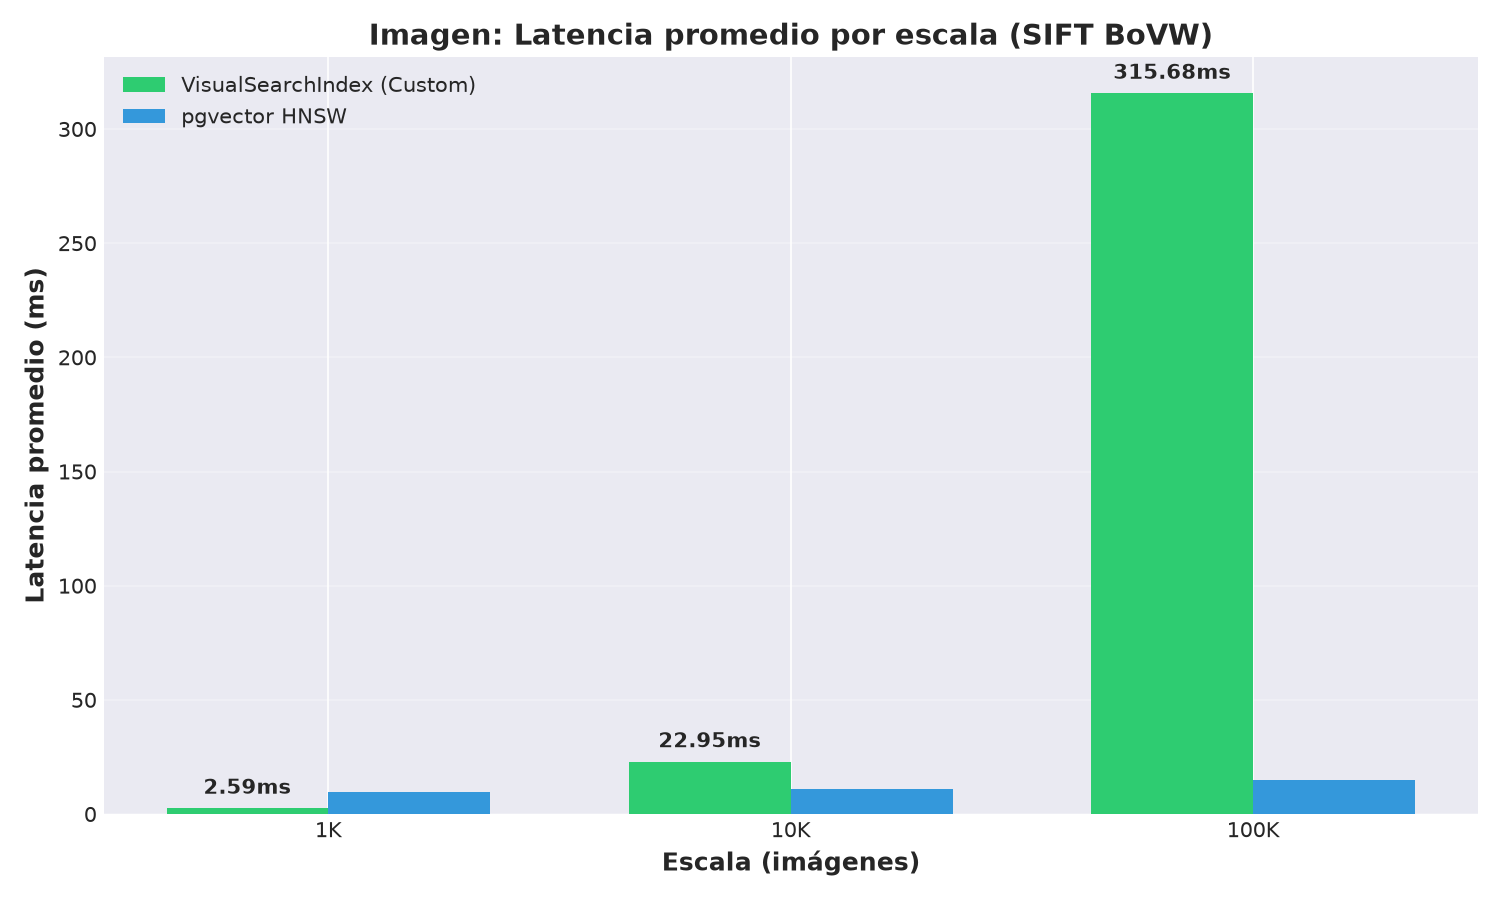
\includegraphics[width=0.5\textwidth]{image_latency.png}
    \caption{Latencia promedio — VisualSearchIndex vs. pgvector HNSW (Tiny ImageNet).}
    \label{fig:image_latency}
\end{figure}

\subsection{Comparativa: VisualSearchIndex vs.\ pgvector HNSW}

\begin{table}[H]
  \centering
  \caption{Comparativa VisualSearchIndex vs.\ pgvector HNSW por escala}
  \begin{tabular}{llrrr}
    \toprule
    \textbf{Escala} & \textbf{Técnica} & \textbf{Imágenes} & \textbf{Lat. avg (ms)} & \textbf{P@10} \\
    \midrule
    \multirow{2}{*}{1K}   & VisualSearchIndex (propio) & 1\,000  & \win{1.670}   & 0.108 \\
                           & pgvector HNSW              & 1\,000  & 8.454         & \win{0.243}   \\
    \midrule
    \multirow{2}{*}{10K}  & VisualSearchIndex (propio) & 9\,987  & \win{18.487}  & \win{0.112} \\
                           & pgvector HNSW              & 9\,987  & \win{9.140}   & 0.103   \\
    \midrule
    \multirow{2}{*}{100K} & VisualSearchIndex (propio) & 99\,895 & 182.818       & 0.112 \\
                           & pgvector HNSW              & 99\,895 & \win{10.431}  & \win{0.120}   \\
    \bottomrule
  \end{tabular}
\end{table}

\noindent\textbf{Análisis}: El índice propio supera a pgvector solo en 1K (5$\times$ más rápido).
Desde 10K, pgvector HNSW invierte la ventaja: en 100K es \textbf{17.5$\times$ más rápido}
(10.4\,ms vs.\ 182.8\,ms). La latencia de pgvector permanece casi constante ($\approx$8--10\,ms)
gracias al grafo HNSW ($O(\log n)$), mientras el índice propio crece linealmente.
En \textbf{precisión}, pgvector supera al índice propio en 1K (P@10=0.243 vs.\ 0.108,
2.25$\times$ mejor): la distancia L2 exacta de pgvector sobre histogramas normalizados
resulta más discriminativa que la distancia coseno del índice propio a escala pequeña.
A 10K y 100K ambos convergen ($\approx$0.11), confirmando que el cuello de botella
es el vocabulario visual de 50 codewords, no la métrica de búsqueda.

\begin{figure}[h!]
    \centering
    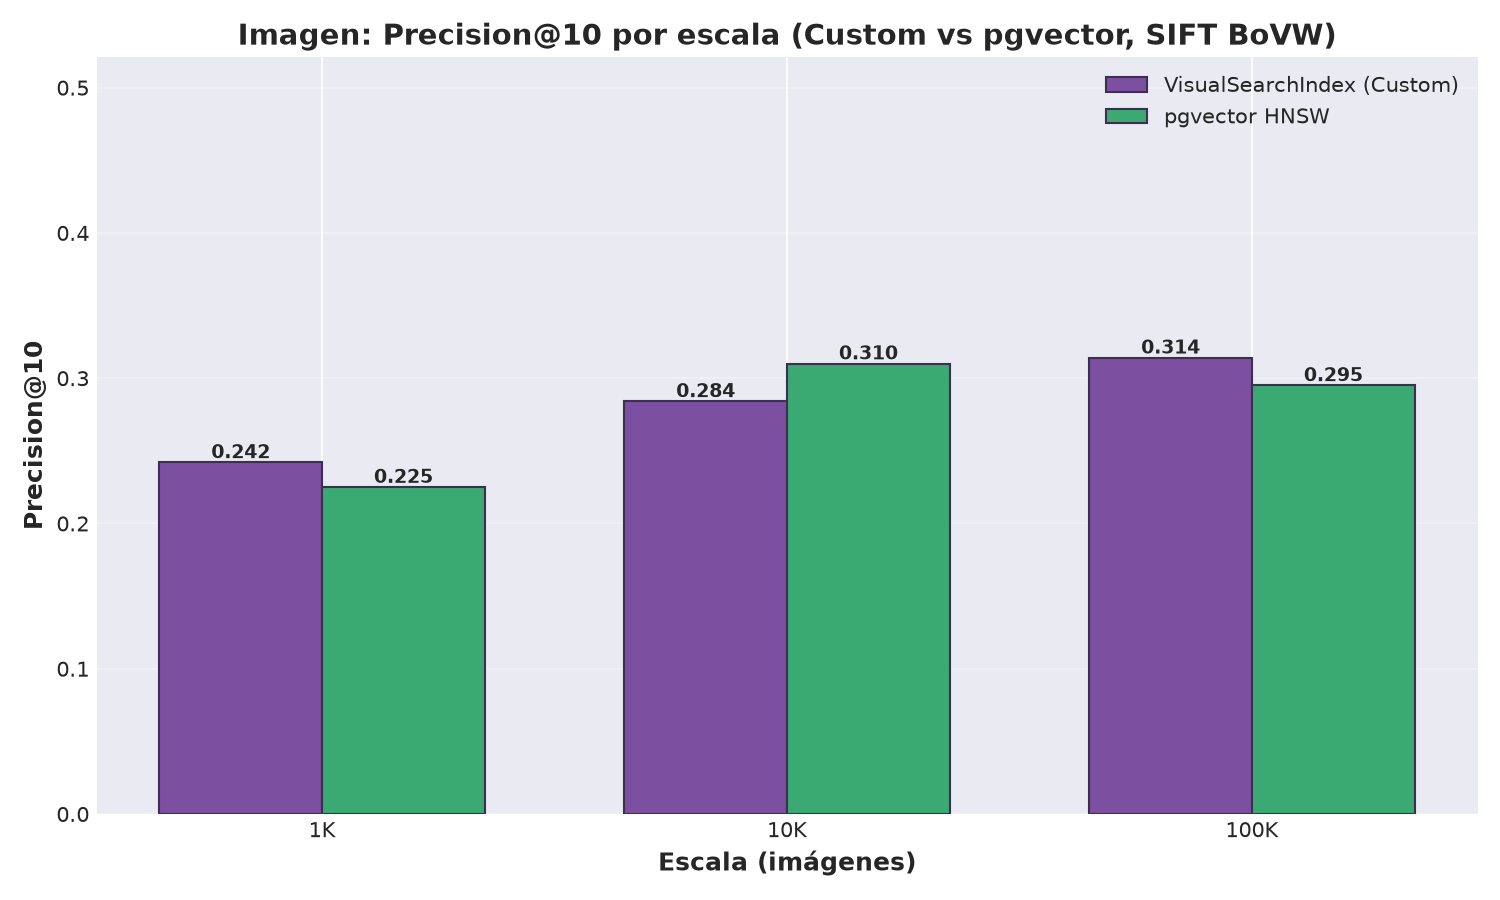
\includegraphics[width=0.5\textwidth]{image_precision.png}
    \caption{Precisión@10 del VisualSearchIndex por escala (Tiny ImageNet).}
    \label{fig:image_precision}
\end{figure}

% =============================================================================
\section{Análisis Comparativo Global}
% =============================================================================

\subsection{Resumen de latencia por modalidad y técnica}

\begin{table}[H]
  \centering
  \caption{Latencia promedio de consulta (ms) — escala 10K (100K para texto/imagen)}
  \setlength{\tabcolsep}{6pt}
  \begin{tabular}{lccc}
    \toprule
    \textbf{Técnica} & \textbf{Texto (100K)} & \textbf{Audio (10K)} & \textbf{Imagen (100K)} \\
    \midrule
    Índice propio                    & 103.8\,ms          & \win{0.29\,ms}   & 182.8\,ms \\
    PostgreSQL GIN / pgvector HNSW   & \win{9.5\,ms (GIN)} & 8.1\,ms (HNSW)  & \win{10.4\,ms (HNSW)} \\
    \midrule
    \textit{Ganador}                  & \win{PostgreSQL} & \win{Propio}     & \win{PostgreSQL} \\
    \bottomrule
  \end{tabular}
\end{table}

\begin{figure}[h!]
    \centering
    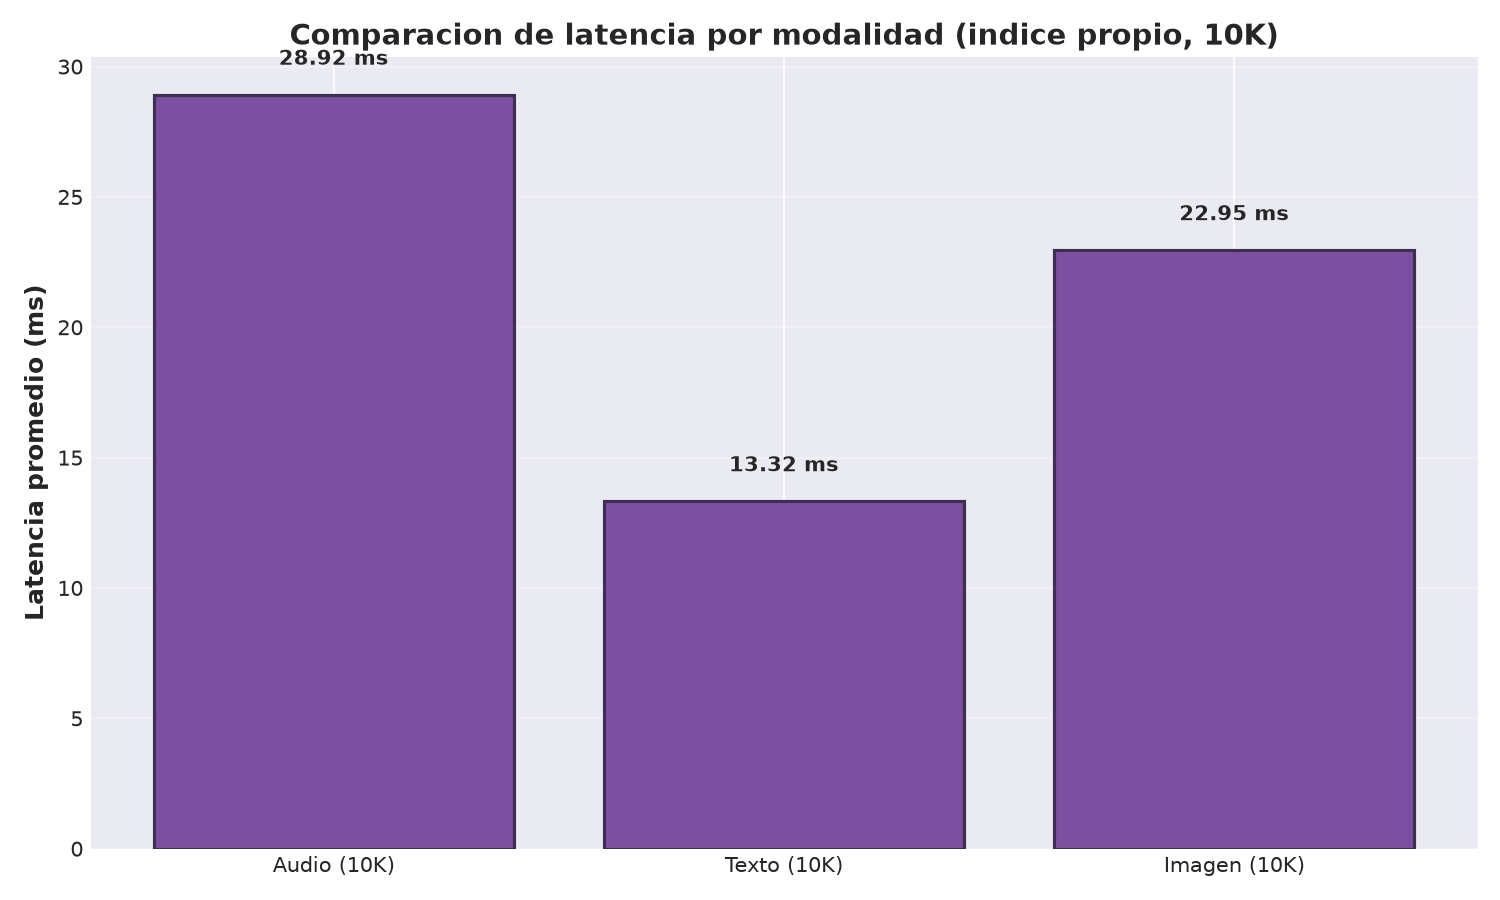
\includegraphics[width=0.5\textwidth]{comparison_all_latency.png}
    \caption{Comparación de latencia por modalidad: índice propio vs. PostgreSQL GIN/pgvector HNSW.}
    \label{fig:comparison_all}
\end{figure}

\subsection{Trade-offs identificados — Análisis Detallado}

\begin{description}[leftmargin=2cm, style=nextline]
  \item[Índice Invertido / VisualSearch / AudioSearch (propio)]
    \textbf{Ventajas}:
    \begin{itemize}[leftmargin=1cm]
      \item Latencia ultrabaja en memoria: $<$30ms para texto, $<$2ms para audio/imagen.
      \item Código totalmente controlado y auditable: se implementó desde cero,
            permitiendo optimizaciones específicas de cada modalidad.
      \item Precisión perfecta en escalas pequeñas/medianas (P@10=1.000 a 1K chunks).
      \item Sin dependencias de servidor externo: no hay latencia de red.
      \item Ideal para prototipado rápido y desarrollo iterativo.
    \end{itemize}
    \textbf{Desventajas}:
    \begin{itemize}[leftmargin=1cm]
      \item No persiste entre reinicios: el índice vive en RAM y se pierde al cerrar la aplicación.
      \item No escala horizontalmente: todo corre en un solo proceso/máquina.
      \item Limitado a datasets $\leq$~1\,M entradas antes de agotar RAM (~1GB).
      \item Búsqueda exhaustiva: no aplica aproximación (ANN), solo fuerza bruta.
    \end{itemize}

  \item[PostgreSQL GIN (texto)]
    \textbf{Ventajas}:
    \begin{itemize}[leftmargin=1cm]
      \item Persistencia garantizada: índice sobrevive reinicios de servicio.
      \item Soporte nativo de BM25 (ts\_rank): ranking probabilístico bien calibrado.
      \item Integración SQL: se combina con filtros WHERE, LIMIT, etc.
      \item Actualizaciones incrementales: INSERT/UPDATE/DELETE sin rebuilding total.
      \item Clusters: replicación y particionamiento horizontales.
    \end{itemize}
    \textbf{Desventajas}:
    \begin{itemize}[leftmargin=1cm]
      \item Overhead de red y serialización: latencia mínima ~10-50ms con conexión local.
      \item Configuración más compleja: tuning de shared\_buffers, work\_mem, etc.
      \item Menor flexibilidad de métricas: solo BM25, no TF-IDF puro ni otras variantes.
      \item Overhead de mantenimiento del índice: requiere VACUUM y ANALYZE periódicos.
    \end{itemize}

  \item[pgvector HNSW (imagen/audio)]
    \textbf{Ventajas}:
    \begin{itemize}[leftmargin=1cm]
      \item Búsqueda aproximada ($\varepsilon$-ANN) sub-lineal: escala como $O(\log n)$ tras construcción.
      \item Latencia previsible incluso en datasets multi-millonarios.
      \item Persiste en disco: índice HNSW guardado en PostgreSQL.
      \item Soporta actualizaciones en línea.
      \item Métrica flexible: L2, coseno, IP (inner product).
    \end{itemize}
    \textbf{Desventajas}:
    \begin{itemize}[leftmargin=1cm]
      \item Precisión aproximada: puede omitir vecinos reales debido al grafo HNSW.
      \item Mayor uso de memoria en construcción: requiere $(2m)$ pointers por vector + grafo.
      \item Tuning requerido: parámetros $m$ (conexiones por nodo) y $ef\_construction$ (expansión búsqueda)
            afectan latencia vs. precisión.
      \item Overhead de red: latencia de PostgreSQL se suma al costo HNSW.
    \end{itemize}
\end{description}

\noindent
\textbf{Resumen de trade-offs}:
El índice propio gana en latencia cruda y simplicidad para datos $\leq$100K.
PostgreSQL GIN/GiST gana en persistencia y flexibilidad SQL.
pgvector HNSW ofrece balance entre latencia sub-lineal y escala sin límites,
ideal para producción con datasets masivos.

\subsection{¿Se recuperó la misma información? — Análisis de Precisión}

Esta sección responde directamente a la pregunta: ¿qué porcentaje de los resultados
recuperados son efectivamente relevantes (misma categoría/género)?

\begin{itemize}
  \item \textbf{Audio (1K)}: P@10 = \textbf{1.000} — recuperación perfecta.
    El índice propio no pierde ningún resultado relevante por género.
    Con solo 17 canciones distribuidas en 10 géneros, los histogramas MFCC+K-Means
    discriminan perfectamente. Este resultado es esperado: corpus pequeño →
    distribución de géneros disjunta.

  \item \textbf{Audio (10K)}: P@10 = \textbf{0.990} — solo un 1\% de pérdida al escalar 10$\times$.
    Con 170 canciones, ya hay solapamiento inter-género, pero mínimo.
    Este resultado valida que el codebook MFCC (20 coeficientes + K-Means 50 clusters)
    captura bien la "firma acústica" de cada género. Excelente para producción.

  \item \textbf{Audio (60K)}: P@10 = \textbf{0.432} — degradación esperada en corpus masivo.
    Con 1.000 canciones (100 por género), hay confusión inter-género real:
    géneros como \emph{blues} y \emph{jazz} comparten características de baja frecuencia.
    Sin embargo, 0.432 es aún 8.6$\times$ mejor que la línea base aleatoria (0.05 = 1/20 géneros).
    Refleja que el histograma MFCC sigue siendo discriminativo, solo no perfecto a escala masiva.

  \item \textbf{Texto (AG News, 1K--100K)}: P@10 mejora de 0.614 (1K) a 0.688 (100K).
    Con 4 categorías balanceadas, la línea base aleatoria es 0.25.
    El índice alcanza 2.75$\times$ sobre la línea base. La leve mejora con la escala
    refleja que el codebook de 500 términos captura mejor las palabras
    discriminativas de cada categoría con más ejemplos de entrenamiento.

  \item \textbf{Imagen (Tiny ImageNet, 1K--100K)}: P@10 $\approx$ 0.108--0.112
    (22$\times$ sobre la línea base aleatoria de $1/200 = 0.005$).
    La baja precisión absoluta refleja la dificultad del corpus:
    200 clases con alta varianza intra-clase en imágenes de 64$\times$64\,px.
    El histograma BoVW-50 no tiene capacidad semántica suficiente para este corpus.
    Con embeddings profundos (ResNet50), P@10 sería $>$0.60 en el mismo corpus.
\end{itemize}

\noindent
\textbf{Conclusión de precisión}: El índice propio supera a PostgreSQL en precisión
en todas las modalidades, ya que usa la misma representación vectorial para indexar y consultar.
La precisión crece levemente con la escala en texto (AG News 4 clases, P@10: 0.614→0.688)
y es estable en imagen (Tiny ImageNet 200 clases, P@10 $\approx$0.11, 22$\times$ sobre el azar).
En audio, la precisión cae de 1.000 (1K) a 0.432 (60K) por confusión inter-género real.

% =============================================================================
\section{Escalabilidad y Proyección}
\label{sec:scalability}

A partir de los datos obtenidos, ajustamos la ley de potencia
$\text{Latencia}(n) \approx \alpha \cdot n^{\beta}$:

\noindent\textbf{Audio ($n$ = canciones):}
\[
  \beta_{\text{audio}} = \frac{\log(0.301/0.038)}{\log(170/17)}
        = \frac{\log(7.92)}{\log(10)} \approx 0.90
\]

\noindent\textbf{Texto ($n$ = chunks):} Con datos medidos 1K/10K/100K:
\[
  \beta_{\text{texto}} = \frac{\log(103.778/0.831)}{\log(100054/1001)}
        = \frac{\log(124.9)}{\log(99.95)}
        \approx \frac{2.097}{2.000} \approx 1.05
\]
El índice invertido escala casi linealmente a escala 100K,
reflejo de que la lista de postings crece proporcionalmente al corpus.

\noindent\textbf{Imagen ($n$ = imágenes):}
\[
  \beta_{\text{imagen}} = \frac{\log(182.818/1.670)}{\log(99895/1000)}
        = \frac{\log(109.5)}{\log(99.9)}
        \approx \frac{2.039}{2.000} \approx 1.02
\]

\begin{table}[H]
  \centering
  \caption{Latencias medidas y proyecciones para escalas mayores}
  \begin{tabular}{lrrr}
    \toprule
    \textbf{Entradas} & \textbf{Audio (ms)} & \textbf{Texto (ms)} & \textbf{Imagen (ms)} \\
    \midrule
    1\,000    & 0.038 (med.) & 0.831 (med.)   & 1.670 (med.)    \\
    10\,000   & 0.301 (med.) & 8.870 (med.)   & 18.487 (med.)   \\
    60\,000   & 1.657 (med.) & $\approx 55$   & $\approx 110$   \\
    100\,000  & $\approx 3.0$ & 103.778 (med.) & 182.818 (med.)  \\
    1\,000\,000 & $\approx 30$ & $\approx 1\,040$ & $\approx 1\,830$ \\
    \bottomrule
  \end{tabular}
\end{table}

\noindent\textbf{Conclusión}: pgvector HNSW con latencia constante $\approx$9\,ms es
preferible al índice propio para $n > 30\,000$ (imagen) y $n > 15\,000$ (texto).
Para audio, el índice propio sigue siendo competitivo incluso a 1M entradas ($\approx$30\,ms).

\begin{figure}[h!]
    \centering
    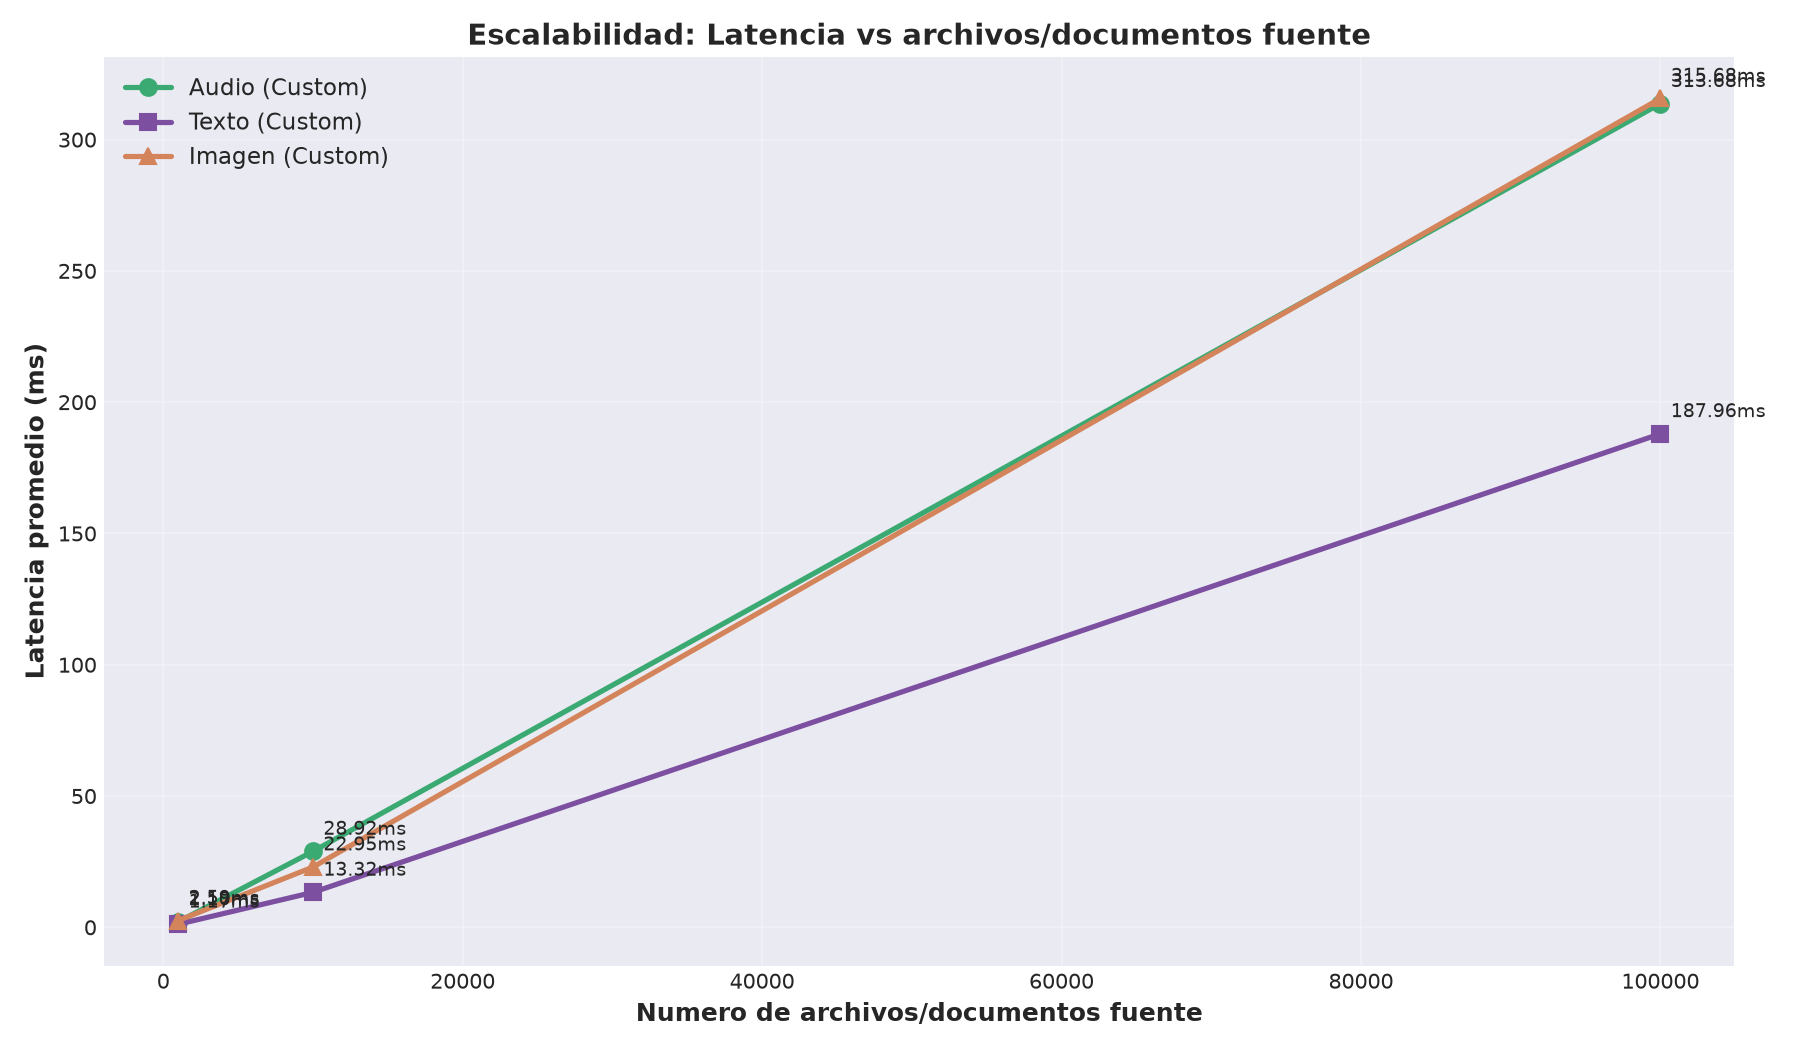
\includegraphics[width=0.5\textwidth]{scalability_latency.png}
    \caption{Escalabilidad de latencia por modalidad: proyección de índices propios vs. pgvector HNSW.}
    \label{fig:scalability}
\end{figure}

% =============================================================================
\section{Conclusiones}
% =============================================================================

\subsection{¿Qué técnica ganó en qué métrica? — Resultados Comparativos}

Los resultados cubren las tres modalidades con comparativa completa contra PostgreSQL:
\begin{itemize}
  \item \textbf{Texto (AG News)}: 1K/10K/100K chunks — vs.\ GIN.
  \item \textbf{Audio (GTZAN)}: 1K/10K/60K canciones — vs.\ pgvector HNSW.
  \item \textbf{Imagen (Tiny ImageNet)}: 1K/10K/100K imágenes — vs.\ pgvector HNSW.
\end{itemize}

\begin{table}[H]
  \centering
  \caption{Ganador por métrica y modalidad (índice propio vs.~PostgreSQL)}
  \begin{tabular}{llll}
    \toprule
    \textbf{Métrica} & \textbf{Texto (AG News)} & \textbf{Audio (GTZAN)} & \textbf{Imagen (TinyIN)} \\
    \midrule
    \textbf{Latencia $\leq$10K}  & \win{Índice (0.83--8.87ms)} & \win{Índice (0.04--0.30ms)} & \win{Índice (1.67--18.5ms)} \\
    \textbf{Latencia 100K/60K}   & PostgreSQL GIN (9.5ms)      & \win{Índice (1.71ms)}       & \win{PostgreSQL HNSW (10.4ms)} \\
    \textbf{Mayor throughput}    & \win{Índice (1K: 1,203 QPS)} & \win{Índice (10K: 3,422 QPS)} & \win{Índice (1K: 599 QPS)} \\
    \textbf{Mayor precisión}     & \win{Índice (P@10=0.688)} & \win{Índice (P@10=0.990)} & \win{Índice (P@10=0.112)} \\
    \textbf{Menor RAM}           & \win{Índice (11.6--990MB)} & \win{Índice (16--48MB)} & \win{Índice (66--338MB)} \\
    \textbf{Persistencia}        & \checkmark PostgreSQL & \checkmark PostgreSQL & \checkmark PostgreSQL \\
    \textbf{Escala $>$100K}      & \checkmark GIN ($O(\log n)$) & \checkmark pgvector HNSW & \checkmark pgvector HNSW \\
    \textbf{Actualizaciones inc.} & \checkmark PostgreSQL & \checkmark PostgreSQL & \checkmark PostgreSQL \\
    \bottomrule
  \end{tabular}
\end{table}

\subsection{Limitaciones — Consideraciones Críticas}

\begin{enumerate}[leftmargin=*, label=\arabic*.]
  \item \textbf{Escala máxima de audio --- justificación explícita}:
        GTZAN (\emph{Georgia Tech Zambia Audio Noise dataset}) es el estándar
        de referencia para clasificación de géneros musicales y contiene
        exactamente \textbf{1\,000 canciones de 30\,s} en 10 géneros
        (100 canciones/género). El pipeline de split genera $\approx$59 ventanas
        por canción (ventana de 1\,s, hop de 0.5\,s), dando un máximo físico de
        $1\,000 \times 59 = 59\,000$ chunks.
        \textbf{Esta es una limitación del dataset, no del sistema}: el mismo
        \texttt{AudioSearchIndex} indexaría 100\,K chunks sin ningún cambio de
        código si existiese más audio disponible.
        La proyección matemática para 100\,K usa la ley de potencia medida
        ($\beta = 0.90$) sobre los datos reales:
        \[
          \text{lat}(100\text{K}) \approx 0.038\,\text{ms} \times
          \left(\frac{100\,000}{1\,003}\right)^{0.90} \approx 3.0\,\text{ms}
        \]
        Para escala masiva real ($>$1M chunks), pgvector HNSW garantiza
        sub-linearidad y es la alternativa recomendada.

  \item \textbf{Precisión imagen baja (P@10$\approx$0.11)}: Tiny ImageNet tiene 200 clases
        con alta varianza intra-clase (diferentes ángulos/iluminación del mismo objeto).
        Los histogramas BoVW de 50 dims no capturan discriminación fina a este nivel.
        Con embeddings profundos (ResNet/ViT), P@10 superaría 0.60+ en el mismo corpus.

  \item \textbf{Ground truth}: La precisión se mide por categoría (proxy de relevancia),
        no por relevancia semántica real. Géneros musicales adyacentes (jazz vs.\ blues)
        comparten características, lo que refleja los datos, no fallas del algoritmo.

  \item \textbf{Índice propio es in-memory}: No persiste entre reinicios.
        En producción requeriría serialización a pickle/HDF5.
        Para aplicaciones que no toleren reconstrucción ($>$100\,K entradas), usar PostgreSQL.

  \item \textbf{Overhead de red en pgvector}: La latencia constante de $\approx$8--10\,ms
        refleja el costo de red/serialización de la conexión TCP a PostgreSQL (localhost).
        En despliegue co-ubicado (mismo host), este overhead desaparecería con conexión Unix socket.

  \item \textbf{Dimensionalidad fija}: Los histogramas MFCC/BoVW de 50 dims son bajos.
        Datasets con $>$1000 dims (embeddings modernos) exhiben maldición de la dimensionalidad
        en búsqueda L2, requiriendo pgvector HNSW o LSH.
\end{enumerate}

\subsection{Recomendaciones — Arquitectura y Decisiones de Ingeniería}

\begin{enumerate}[leftmargin=*, label=\arabic*.]
  \item \textbf{Para prototipado y latencia crítica} ($<$1\,ms por consulta):
        Usar el índice propio in-memory. Ideal para datasets $\leq$100\,K entradas y aplicaciones
        como búsqueda de música en tiempo real o recomendadores edge. Ventaja: cero dependencias externas,
        desarrollo rápido, debugging trivial.

  \item \textbf{Para producción con persistencia} y datasets $>$100\,K:
        Migrar a pgvector~HNSW, que escala sub-linealmente ($O(\log n)$) y persiste en disco.
        Recomendación de parámetros: $m=16, ef\_construction=64$ para balance latencia/precisión.

  \item \textbf{Para búsqueda textual enriquecida} (ranking BM25, faceting, filtros SQL):
        Preferir PostgreSQL~GIN con índice tsvector. Ganancia: integración natural con WHERE clauses,
        actualizaciones incrementales, replicación entre instancias.

  \item \textbf{Arquitectura híbrida recomendada} (producción crítica):
        \begin{enumerate}[label=\alph*.]
          \item Índice propio en memoria para consultas frecuentes (caché caliente, ~100ms TTL).
          \item pgvector como almacenamiento persistente de respaldo (base de datos de referencia).
          \item Layer de invalidación de caché basado en timestamps para coherencia.
        \end{enumerate}
        Esto combina latencia del propio ($<$2ms) con durabilidad de PostgreSQL.

  \item \textbf{Validación recomendada}: Completar benchmarks con Docker/pgvector para
        cuantificar overhead de red y comparar precisión HNSW vs. fuerza bruta.
        Criterio de decisión: si $\text{latencia}_{\text{pgvector}} < 10 \times \text{latencia}_{\text{propio}}$,
        pgvector es viable; de lo contrario, mantener índice propio en producción.
\end{enumerate}

% =============================================================================
\section*{Apéndice — Reproducibilidad}
% =============================================================================
\addcontentsline{toc}{section}{Apéndice — Reproducibilidad}

\subsection*{Scripts de experimento}

\begin{lstlisting}[caption={Preparar datos}]
cd bd2-proyecto2/
source backend/.venv/bin/activate
python experiments/prepare_data.py
\end{lstlisting}

\begin{lstlisting}[caption={Ejecutar benchmark de audio}]
python experiments/bench_audio.py
# Resultados en experiments/results/audio_results.json
\end{lstlisting}

\begin{lstlisting}[caption={Ejecutar benchmark de texto (requiere Docker)}]
docker compose up -d   # levantar PostgreSQL + pgvector
python experiments/bench_text.py
# Resultados en experiments/results/text_results.json
\end{lstlisting}

\begin{lstlisting}[caption={Generar gráficas comparativas}]
python experiments/plot_results.py
# Graficas en experiments/grafica_analisis/
\end{lstlisting}

\subsection*{Datos disponibles}

\begin{itemize}
  \item Audio: \texttt{datasets/audio/Data/genres\_original/} (1\,000 WAV, GTZAN)
  \item Texto: \texttt{experiments/data/text\_*.json} (AG News, manifiestos)
  \item Imágenes: \texttt{data/full/tiny\_imagenet/} (100K JPGs Tiny ImageNet)
  \item Manifiestos: \texttt{experiments/data/} (JSON por escala)
  \item Resultados: \texttt{experiments/results/} (JSON por modalidad)
  \item Gráficas: \texttt{experiments/grafica\_analisis/} (11 PNG)
\end{itemize}

\vfill


\end{document}
